% Für Bindekorrektur als optionales Argument "BCORfaktormitmaßeinheit", dann
% sieht auch Option "twoside" vernünftig aus
% Näheres zu "scrartcl" bzw. "scrreprt" und "scrbook" siehe KOMA-Skript Doku
\documentclass[12pt,a4paper,titlepage,headinclude,bibtotoc]{scrartcl}


%---- Allgemeine Layout Einstellungen ------------------------------------------

% Für Kopf und Fußzeilen, siehe auch KOMA-Skript Doku
\usepackage[komastyle]{scrpage2}
\pagestyle{scrheadings}
\setheadsepline{0.5pt}[\color{black}]
\automark[section]{chapter}


%Einstellungen für Figuren- und Tabellenbeschriftungen
\setkomafont{captionlabel}{\sffamily\bfseries}
\setcapindent{0em}


%---- Weitere Pakete -----------------------------------------------------------
% Die Pakete sind alle in der TeX Live Distribution enthalten. Wichtige Adressen
% www.ctan.org, www.dante.de

% Sprachunterstützung
\usepackage[ngerman]{babel}

% Benutzung von Umlauten direkt im Text
% entweder "latin1" oder "utf8"
\usepackage[utf8]{inputenc}

% Pakete mit Mathesymbolen und zur Beseitigung von Schwächen der Mathe-Umgebung
\usepackage{latexsym,exscale,stmaryrd,amssymb,amsmath}

% Weitere Symbole
\usepackage[nointegrals]{wasysym}
\usepackage{eurosym}

% Anderes Literaturverzeichnisformat
%\usepackage[square,sort&compress]{natbib}
\usepackage{hyperref}
% Für Farbe
\usepackage{color}

% Zur Graphikausgabe
%Beipiel: \includegraphics[width=\textwidth]{grafik.png}
\usepackage{graphicx}

% Text umfließt Graphiken und Tabellen
% Beispiel:
% \begin{wrapfigure}[Zeilenanzahl]{"l" oder "r"}{breite}
%   \centering
%   \includegraphics[width=...]{grafik}
%   \caption{Beschriftung} 
%   \label{fig:grafik}
% \end{wrapfigure}
\usepackage{wrapfig}

% Mehrere Abbildungen nebeneinander
% Beispiel:
% \begin{figure}[htb]
%   \centering
%   \subfigure[Beschriftung 1\label{fig:label1}]
%   {\includegraphics[width=0.49\textwidth]{grafik1}}
%   \hfill
%   \subfigure[Beschriftung 2\label{fig:label2}]
%   {\includegraphics[width=0.49\textwidth]{grafik2}}
%   \caption{Beschriftung allgemein}
%   \label{fig:label-gesamt}
% \end{figure}
\usepackage{subfigure}

% Caption neben Abbildung
% Beispiel:
% \sidecaptionvpos{figure}{"c" oder "t" oder "b"}
% \begin{SCfigure}[rel. Breite (normalerweise = 1)][hbt]
%   \centering
%   \includegraphics[width=0.5\textwidth]{grafik.png}
%   \caption{Beschreibung}
%   \label{fig:}
% \end{SCfigure}
\usepackage{sidecap}

% Befehl für "Entspricht"-Zeichen
\newcommand{\corresponds}{\ensuremath{\mathrel{\widehat{=}}}}
% Befehl für Errorfunction
\newcommand{\erf}[1]{\text{ erf}\ensuremath{\left( #1 \right)}}

%Fußnoten zwingend auf diese Seite setzen
\interfootnotelinepenalty=1000

%Für chemische Formeln (von www.dante.de)
%% Anpassung an LaTeX(2e) von Bernd Raichle
\makeatletter
\DeclareRobustCommand{\chemical}[1]{%
  {\(\m@th
   \edef\resetfontdimens{\noexpand\)%
       \fontdimen16\textfont2=\the\fontdimen16\textfont2
       \fontdimen17\textfont2=\the\fontdimen17\textfont2\relax}%
   \fontdimen16\textfont2=2.7pt \fontdimen17\textfont2=2.7pt
   \mathrm{#1}%
   \resetfontdimens}}
\makeatother

%Honecker-Kasten mit $$\shadowbox{$xxxx$}$$
\usepackage{fancybox}

%SI-Package
\usepackage{siunitx}

%keine Einrückung, wenn Latex doppelte Leerzeile
\parindent0pt

%Bibliography \bibliography{literatur} und \cite{gerthsen}
%\usepackage{cite}
\usepackage{babelbib}
\selectbiblanguage{ngerman}

\begin{document}

\begin{titlepage}
\centering
\textsc{\Large Anfängerpraktikum der Fakultät für
  Physik,\\[1.5ex] Universität Göttingen}

\vspace*{3cm}

\rule{\textwidth}{1pt}\\[0.5cm]
{\huge \bfseries
  Fresnelsche Formeln\\[1.5ex]
  und Polarisation}\\[0.5cm]
\rule{\textwidth}{1pt}

\vspace*{3cm}

\begin{Large}
\begin{tabular}{ll}
Praktikant: &  Michael Lohmann\\
Versuchspartner: &  Felix Kurtz\\
 E-Mail: & m.lohmann@stud.uni-goettingen.de\\
 Betreuer: & Phillip Bastian\\
 Versuchsdatum: & 06.03.2015\\
\end{tabular}
\end{Large}

\vspace*{0.8cm}

\begin{Large}
\fbox{
  \begin{minipage}[t][2.5cm][t]{6cm} 
    Eingegangen am:
  \end{minipage}
}
\end{Large}

\end{titlepage}

\tableofcontents

\newpage

\section{Einleitung}
\label{sec:einleitung}
Elektromagnetische Strahlung in Form von Licht ist essentiel für die Entstehung von Leben, da es die größte Energiequelle auf Planeten darstellt.
Eine der Eigenschaften von EM-Strahlung ist die Polarisation.
Sie wird in technischen Geräten wie dem 3D-Kino verwendet, findet aber auch Anwendung in der Fotografie.
Möchte man einen See fotografieren, so hat man meist störende Reflektionen an der Oberfläche, welche sich mit einem Polarisationsfilter minimieren lassen.
Dieses Verhalten soll in diesem Versuch untersucht werden.

\section{Theorie}
\label{sec:theorie}
\subsection{Polarisation}
Die \textit{Maxwellschen}-Gleichungen, welche die Ausbreitung von elektro-magnetischen Wellen beschreiben, lassen Polarisation zu, da es ich bei ihnen um Transversalwellen handelt.
Das bedeutet, dass das $\vec E$- und das $\vec B$-Feld bestimmte Phasenbeziehungen haben können.
Die Polarisation lässt sich darstellen durch einen Vektor, der senkrecht auf der Ausbreitungsrichtung steht, wesshalb zwei Koordinaten zur Beschreibung reichen.
Das meiste Licht wird durch statistische Vorgänge wie die Emission eines Photons bei der Relaxation eines angeregten Elektrons erzeugt.
Daher hat es keine ausgezeichnete Polarisationsrichtung.
Unter bestimmten Bedingungen kann jedoch eine bestimmte Polarisationsrichtung herausgefiltert werden.

Es gibt drei verschiedene Fälle:
\begin{itemize}
	\item Linear: Der Feldvektor zeigt konstant in eine Richtung und verändert dabei periodisch seinen Betrag.
	\item Elliptisch: Der Feldvektor rotiert periodisch um den Wellenvektor und verändert dabei periodisch seinen Betrag.
	\item Zirkular: Wie elliptisch, nur dass der Betrag erhalten bleibt.
\end{itemize}

Man kann jeden Feldvektor in zwei senkrecht aufeinander stehende Schwingungen zerlegen.
Sind die beiden in Phase, so ist es linear polarisiertes Licht, wohingegen es bei einem Phasenverschub von $\frac{\pi}{2}$ zirkulares Licht darstellt.

Man kann bei Reflektionen die beiden Schwingungen so zerlegen, dass eine in der Einfallsebene liegt und eine senkrecht dazu.
Diese nennt man dann parallel ($E_p$) und senkrecht ($E_s$).

\subsection{Reflektion an Grenzflächen}
Nach dem \textit{Snellnius}'schen Brechungsgesetz gilt für die Brechung an einer Oberfläche
\begin{align}
	n_1\cdot\sin\alpha=n_2\cdot\sin\beta
\end{align}
wobei $n_i$ der jeweilige Brechungsindex ist und $\alpha$ der Ein- sowie $\beta$ der Ausfallwinkel des Lichts ist.
Da der Sinus jedoch beschränkt ist, kann für einen Übergang vom optisch dichteren ins dünnere ($n_1 > n_2$) ab einem bestimmten kritischen Winkel kein Licht mehr transmitieren.
Der Übergang ist jedoch nicht schlagartig, sondern folgt nach \cite[S. 238]{demtroeder2} den \textsc{Fresnellschen Formeln}:
\begin{align}
	r_s &= -\frac{\sin (\alpha -\beta )}{\sin ( \alpha + \beta )}\\
	r_p &= \frac{\tan (\alpha - \beta )}{\tan ( \alpha + \beta )}\\
	t_s &= \frac{2\sin\alpha\sin\beta}{\sin (\alpha +\beta )}\\
	t_p &= \frac{2\sin\beta\cos\alpha}{\sin ( \alpha + \beta )\cos(\alpha - \beta)}\, .
\end{align}
Die Reflektionskoeffizienten $r_s$ und $r_p$ sind in Abb. \ref{fig:reflektion} abgebildet.


\begin{figure}[h]
	\centering
	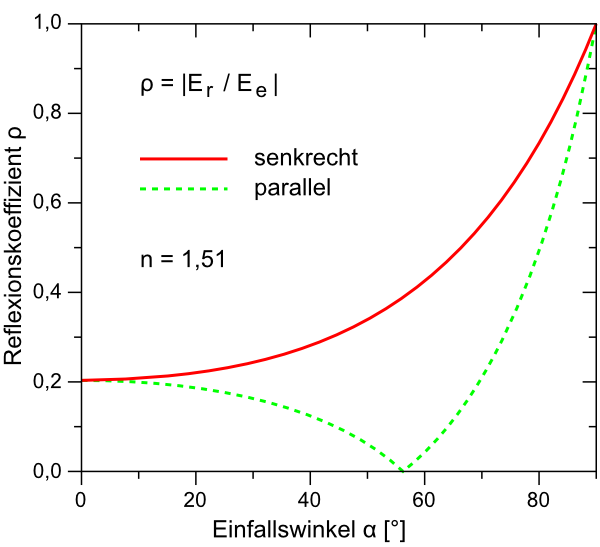
\includegraphics{fresnelkoeff_lp}
	\caption{Reflektionskoeffizienten aufgetragen gegen den Einfallswinkel nach \cite[28.3.2015, 15 Uhr]{lp20}}
	\label{fig:reflektion}
\end{figure}
\section{Durchführung}
\label{sec:durchfuehrung}
Für den Versuch wird eine optische Schiene wie in Abb. \ref{fig:schiene} verwendet, welche sich am Anfang gerade auf $0^\circ $  befindet.
Nachdem die Quecksilberdampflampe angeschaltet wurde und die Intensität ausreicht, kann nun begonnen werden, den Strahlengang einzustellen.
Die sich auf der Schiene befindenden Linsen müssen zunächst ohne das Prisma so abgestimmt werden, dass das (nahc dem Filter grüne) Lichtbündel scharf in dem Okular erkennbar ist.
Dafür werden Polarisator und Analysator so eingestellt, dass sie alles Licht durchlassen.
Um die Polarisationsrichtung korrekt einzustellen wird nun das Nicol-Prisma auf den Drehteller gestellt.
Die Standfläche ist dabei so ausgerichtet, dass die optische Achse vertikal zur Strahlrichtung liegt.
Ohne den Analysator im Strahlengang wird nun der Polarisator auf maximalen Durchlass gestellt.
%Da das menschliche Auge Helligkeitsunterschiede wesentlich deutlicher wahrnimmt, wenn die Gesamthelligkeit gering ist, empfielt es sich, zunächst den Punkt der absoluten Dunkelheit zu suchen und dann den Polarisator um $90^\circ$ zu verdrehen.
Für die erste Messung wird nun der Polarisator so eingestellt, dass keine Helligkeit mehr sichtbar ist (was einer Polarisation parallel zur Einfallsebene entspricht) und dann um $45^\circ$ verdreht.
Nun wird das Nicol-Prisma durch ein Glasprisma ersetzt, welches in der $0^\circ$-Lage der Schiene genau im und parallel zum Strahlengang steht.
Auf den Drehtellern befinden sich zumeist schon Markierungen, welche  dadurch überprüft werden können, dass der Strahl bis zu einer Auslenkung von $90^\circ$ der optischen Schiene durch das Okular sichtbar sein muss.

Um nun den Reflektionskoeffizienten zu vermessen wird nun der Analysator erneut in den Strahlengang gestellt.
Er wird nun, während die Schiene in je $5^\circ$-Schritten weiter gestellt wird, in die Position gestellt, dass kein Licht mehr durchgelassen wird.
Die beiden Winkel werden notiert.

Zur Ermittlung des Brewster-Winkels werden nun der Polarisator wieder um $45^\circ$ zurück gedreht und der Analysator entfernt.
Dann wird der Auslenkwinkel der Schiene gesucht und notiert, bei welcher die geringste Intensität zu sehen ist.
Hierbei empfielt es sich, abwechseld mit dem Versuchspartner die Messung durchzuführen.


\section{Auswertung}
\label{sec:auswertung}


\section{Diskussion}
\label{sec:diskussion}


\bibliography{literatur} 
\bibliographystyle{babalpha} 
\end{document}
